\begin{tikzpicture}%
\def\lx{0.5*\linewidth}%
\node[inner sep=0pt] (heat) at (-0.5,0) {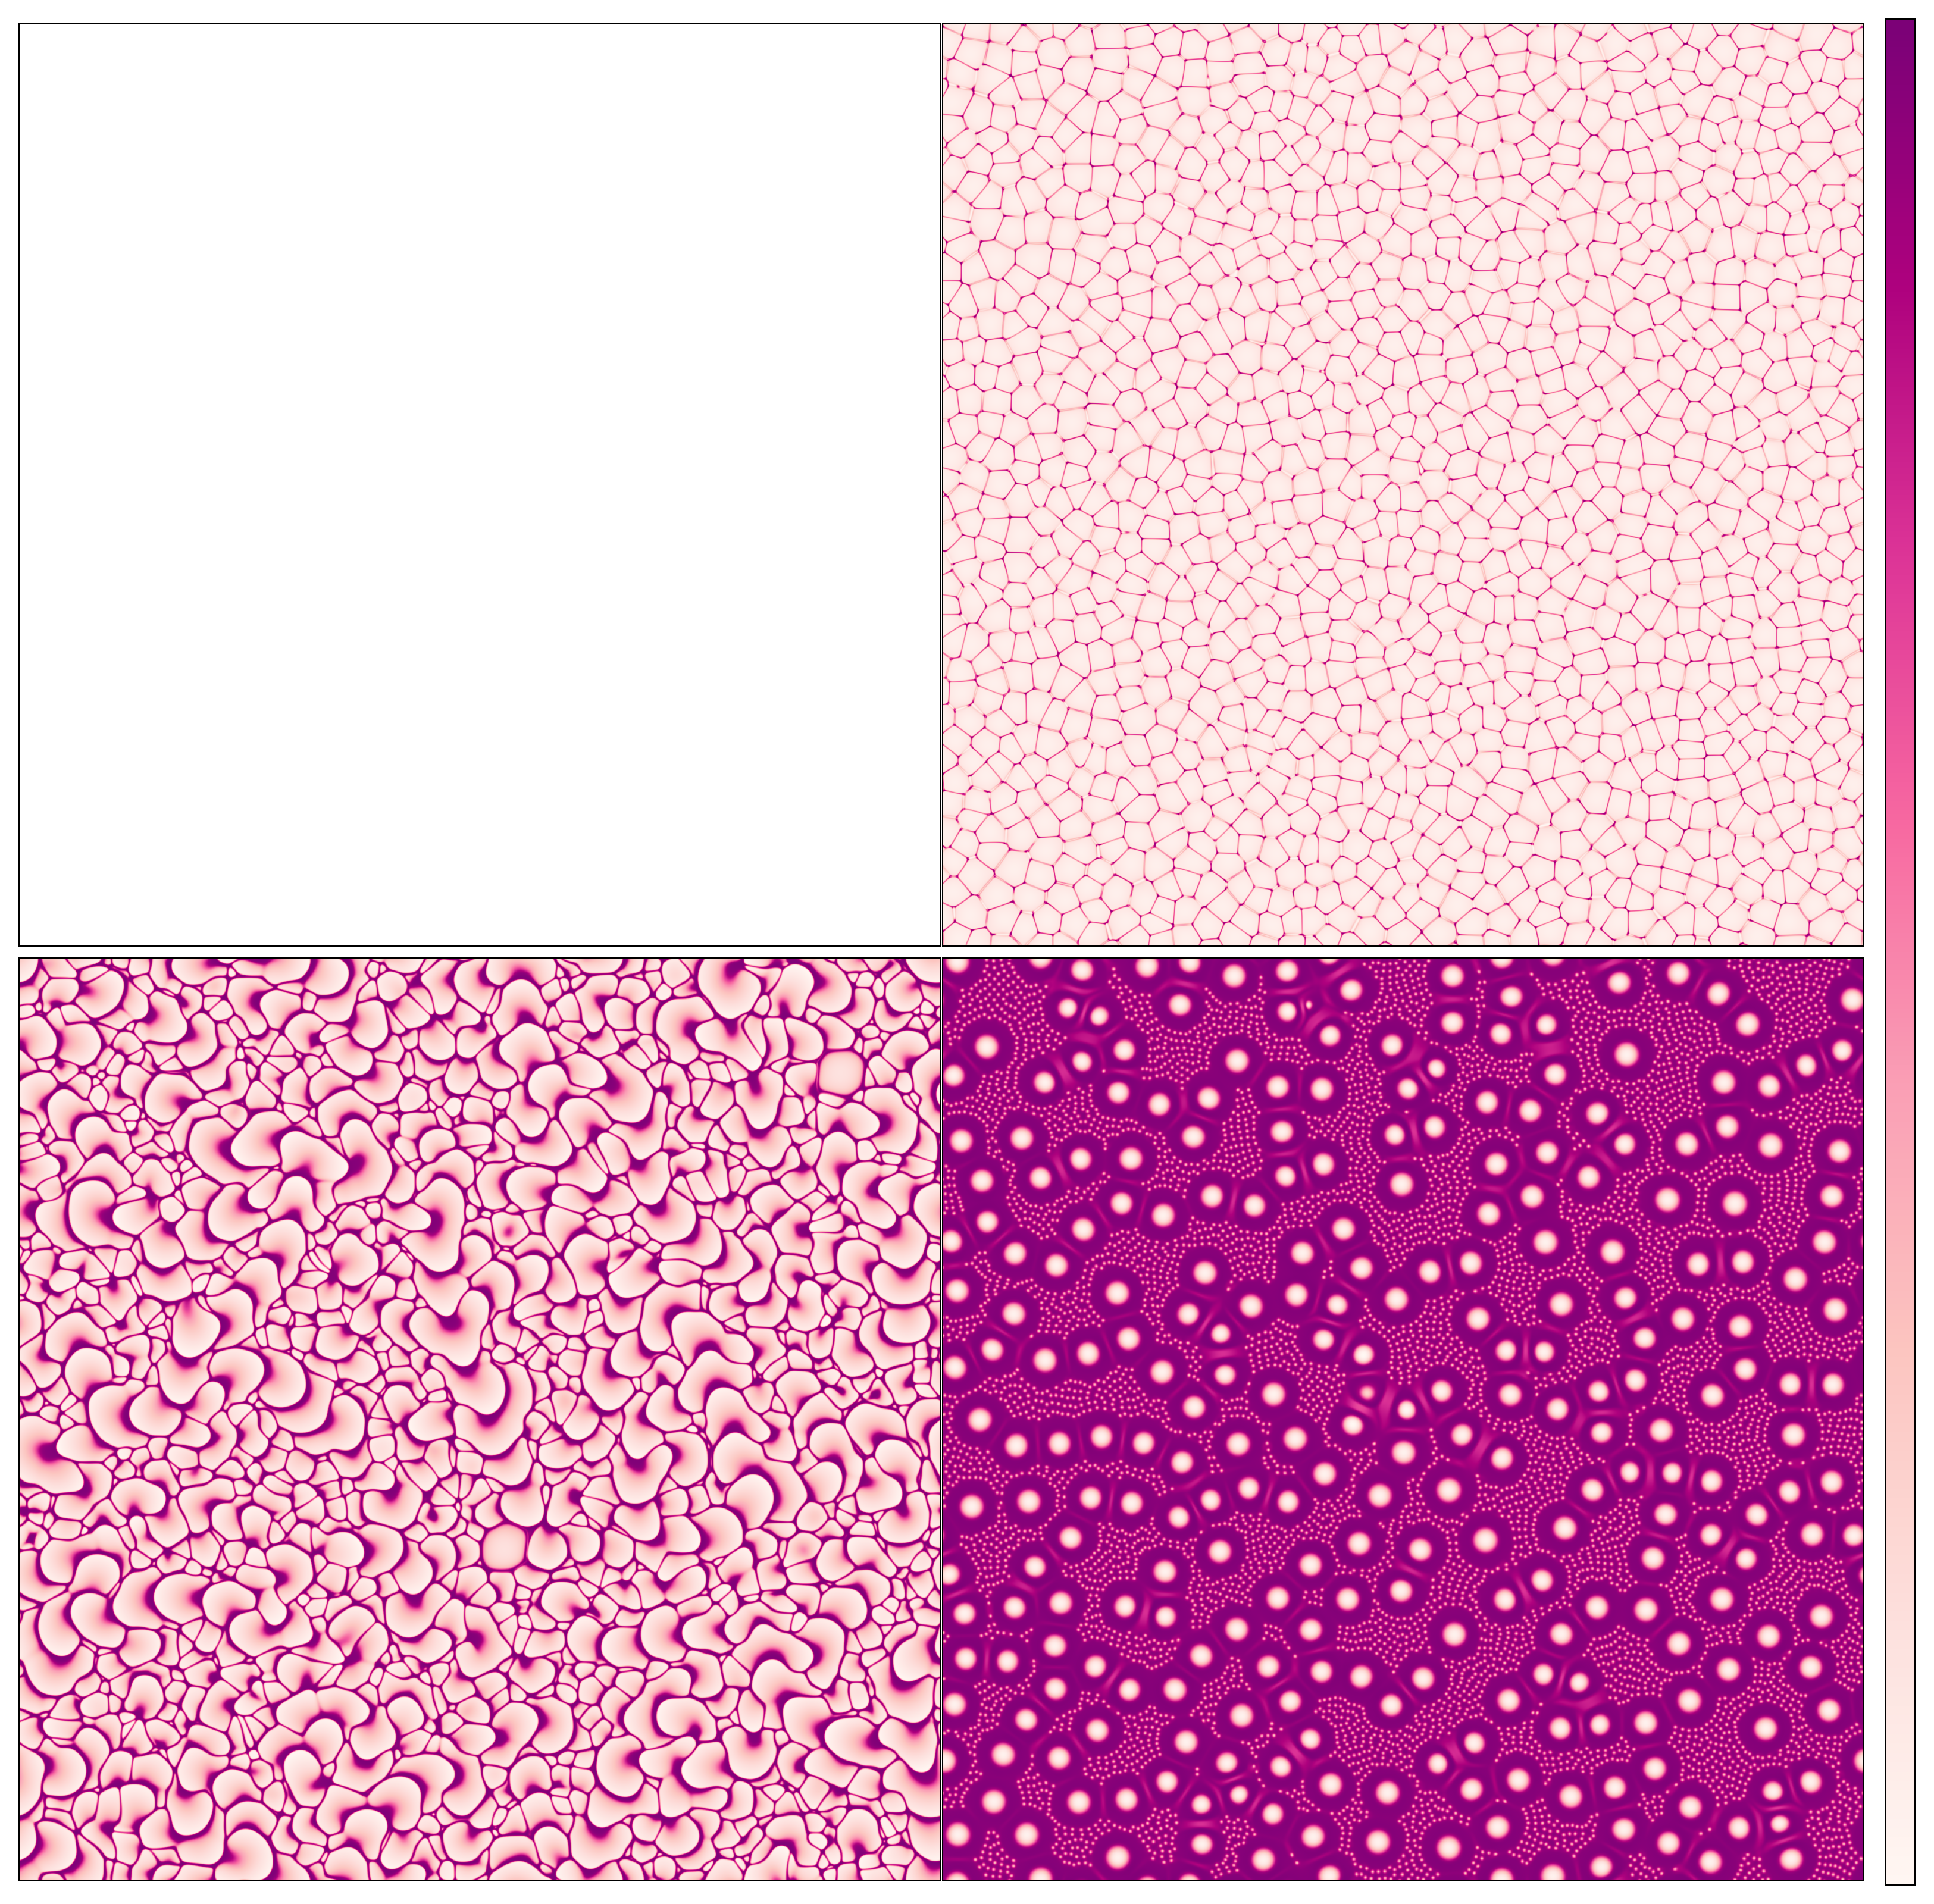
\includegraphics[width=0.9\linewidth]{phases_L50_3.png}};

\node at (0.89*\lx,-0.85*\lx) {$\rho_{min}$};
\node at (0.89*\lx,0.85*\lx) {$\rho_{max}$};
\node at (0.89*\lx,0) {$\rho$};

\node[text = black, rectangle, rounded corners=3pt, fill=white, opacity=0.85] at (-0.89*\lx, 0.82*\lx) {(a)};
\node[text = black, rectangle, rounded corners=3pt, fill=white, opacity=0.85] at (-0.02*\lx, 0.82*\lx) {(b)};
\node[text = black, rectangle, rounded corners=3pt, fill=white, opacity=0.85] at (-0.89*\lx, -0.05*\lx) {(c)};
\node[text = black, rectangle, rounded corners=3pt, fill=white, opacity=0.85] at (-0.02*\lx, -0.05*\lx) {(d)};

% Turnover
\fill[color=RdPu1] (-0.87*\lx,0.48*\lx) rectangle ++ (0.12*\lx,0.12*\lx);
\node[align=center] at (-0.81*\lx, 0.54*\lx) {$\rho<\rho_0$};
\draw[->, thick, >=stealth] (-0.75*\lx,0.54*\lx) -- ++(0.1*\lx,0);
\fill[color=RdPu2] (-0.65*\lx,0.48*\lx) rectangle ++ (0.12*\lx,0.12*\lx);
\node[align=center] at (-0.59*\lx, 0.54*\lx) {$\rho_0$};

\fill[color=RdPu3!70!RdPu2] (-0.87*\lx,0.62*\lx) rectangle ++ (0.12*\lx,0.12*\lx);
\node[align=center] at (-0.81*\lx, 0.68*\lx) {$\rho>\rho_0$};
\draw[->, thick, >=stealth] (-0.75*\lx,0.68*\lx) -- ++(0.1*\lx,0);
\fill[color=RdPu2] (-0.65*\lx,0.62*\lx) rectangle ++ (0.12*\lx,0.12*\lx);
\node[align=center] at (-0.59*\lx, 0.68*\lx) {$\rho_0$};

\node[align=center] at (-0.70*\lx,0.61*\lx) {$t\sim\tau$};
\node[align=center] at (-0.70*\lx,0.40*\lx) {\footnotesize renewal};

% Active stress
\fill[color=RdPu2] (-0.38*\lx,0.55*\lx) rectangle ++ (0.16*\lx,0.16*\lx);
\node[align=center] at (-0.3*\lx,0.63*\lx) {$\zeta_\rho\rho^3\Delta\mu$};
\draw[<-, color=ao, ultra thick, >=stealth] (-0.38*\lx,0.63*\lx)--(-0.45*\lx,0.63*\lx);
\draw[<-, color=ao, ultra thick, >=stealth] (-0.22*\lx,0.63*\lx)--(-0.15*\lx,0.63*\lx);
\draw[<-, color=ao, ultra thick, >=stealth] (-0.3*\lx,0.55*\lx)--(-0.3*\lx,0.48*\lx);
\draw[<-, color=ao, ultra thick, >=stealth] (-0.3*\lx,0.71*\lx)--(-0.3*\lx,0.78*\lx);
\node[align=center] at (-0.3*\lx,0.40*\lx) {\footnotesize active stress};

% Density-polarity Coupling
\node[align=center] at (-0.5*\lx,0.05*\lx) {\footnotesize density-polarity coupling ($p^2 \sim \rho/\rho_0$)};
\shade[left color=RdPu1, right color=RdPu3, middle color=RdPu2] (-0.8*\lx,0.1*\lx) rectangle ++ (0.6*\lx,0.2*\lx);
\draw[->, >=latex, ultra thick] (-0.7*\lx,0.17*\lx) -- (-0.7*\lx,0.23*\lx);
\draw[->, >=latex, ultra thick] (-0.5*\lx,0.15*\lx) -- (-0.5*\lx,0.25*\lx);
\draw[->, >=latex, ultra thick] (-0.3*\lx,0.13*\lx) -- (-0.3*\lx,0.27*\lx);
\end{tikzpicture}